\section{ARCHITECTURAL DESIGN}
\subsection{Overview} 
In this section is provided a complete overview of all the system components, from the logical level to the physical level of the PowerEnJoy service. First of all we give a description of the high level components and their interaction.\newline

\noindent From an high level prospective the service is composed by different modules allowing development and maintenance flexibility.This modularity allow also scalability for future service expansion, \todo{espandere il concetto} \newline


\begin{itemize}
\item{\textbf{Database:}} the data layer of the service. All the persistent data will be stored in this layer.
\item{\textbf{Application Server:}} this component will manage the applicative logic.
\item{\textbf{Web Server:}} this layer is the interface with the world. It will manage the requests from the users and the website.
\item{\textbf{Mobile Application Interface:}} this is the interface between the Mobile User and the system. The user will use it to send requests to the web Server and see the results sent back through his mobile device. 
\item{\textbf{Car OnBoard Device:}} this is the module mounted on the car. It will communicate with the server and with the car ECU.
\item{\textbf{Web Site Interface:}} this is the interface between the Web User and the system.The user will use it to send requests to the web Server and see the results sent back through the web site. 
\end{itemize}

	\begin{figure}[H]	
	\centering
	\includegraphics[scale=0.5]{img/architecture_diagram}
	\caption{Architecture Diagram}
\end{figure}


\newpage
\subsection{Component view} 
From a lower level perspective, the components of the system are:
\todo{Dubbio: Cosa va nel Web Server?}

\begin{itemize}
\item User Web Client GUI:
\item User Mobile Client GUI:
\item Driver Client GUI:
\item Data Manager:
\item Request Manager:
\item Account Manager:
\item Position Manager:
\item Travel Manager:


\end{itemize}
The communication between the clients (both mobile application and web site) are realized using a request-response methodology. The client ask for information or make action related to the server using \textbf{REST} requests and obtain a response from the server formatted as a \textbf{JSON} object, today the state of the art for web services communications.
All the REST requests received by the \textbf{HTTP Server} are processed by the Request Handler component. The Request Handler component is in charge of validate the request integrity, parse it using the \textbf{REST Parser }component and check the authentication for the requests type that need a valid session.


When a requests pass those check is forwarded to the Service Manager where the application logic is applied.
The \textbf{Service Manager} in base of what request are received process a response using Car Manager, User Manager, Position Manager and Trip Manager.
Using those component the Service Manager can access the model, manage the request and craft a response.Every request can instantiate different component,


The system status are represented through various \textbf{Java Beans} object that stay alive for all the time needed for the request processing.

	\begin{figure}[H]	
	\centering
	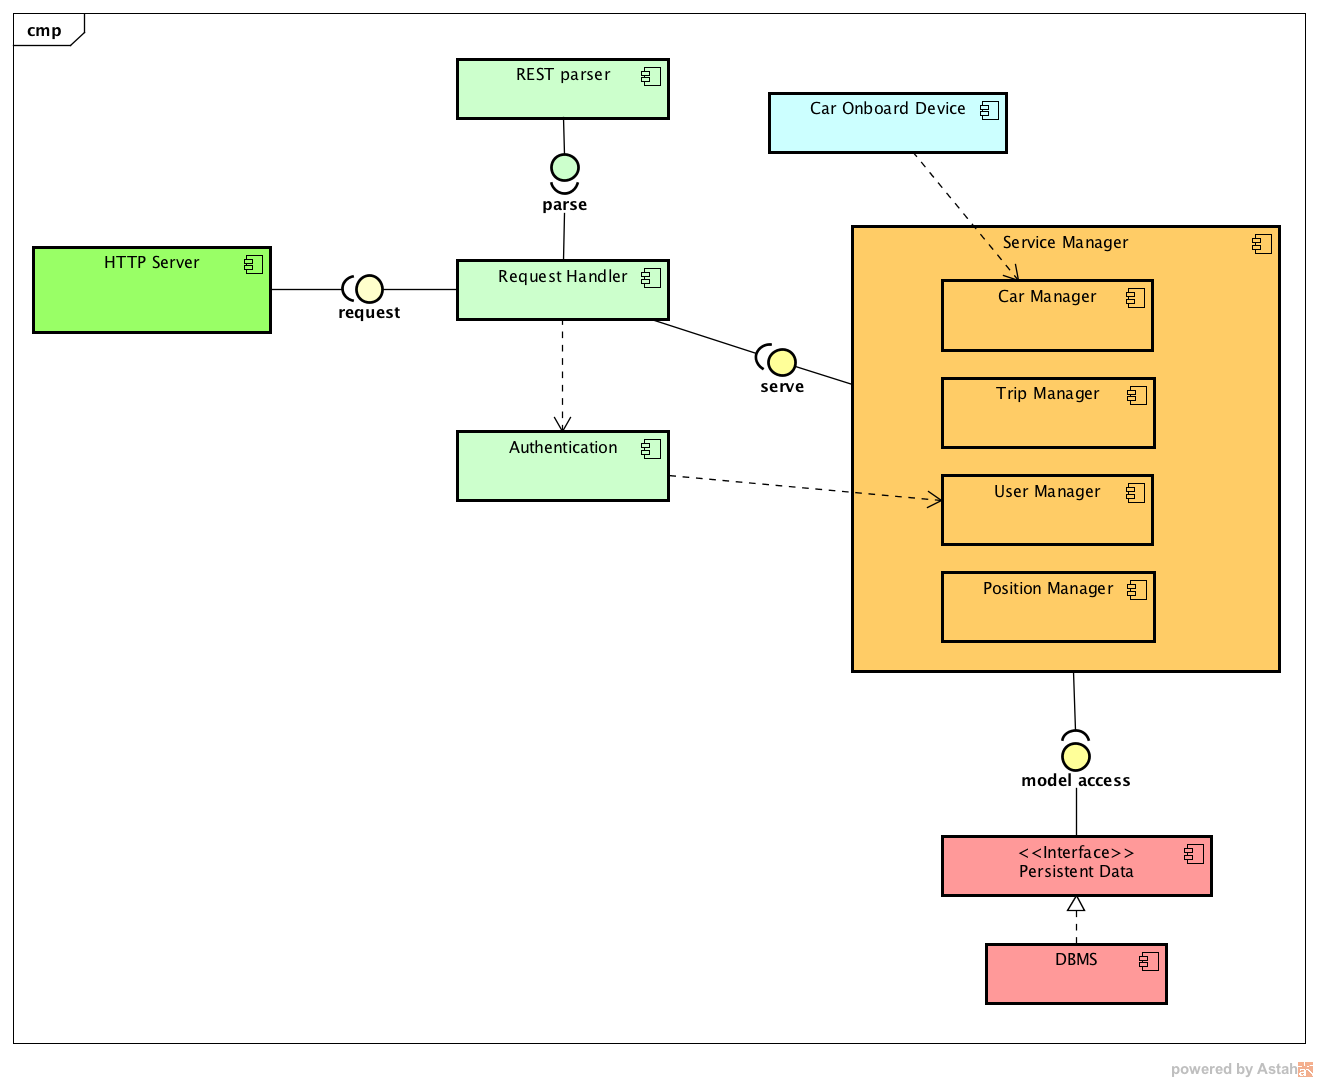
\includegraphics[width=\textwidth]{img/backend_component_diagram}
	\caption{Back-End Component Diagram}
\end{figure}

When a request is received all the element from the model needed for the processing are loaded from the persistent data storage through the \textbf{Persistent Data interface}. The abstraction exposed by the Persistent Data interface allow to adopt different data storage solution in a transparent way to the various component that are using it. All the persistent data are stored through a distributed database that can optimize data access.

The \textbf{Position Manager} implements the logic for the manage of the position and the distance between cars, users and safe area. It also handle which cars show to the user in base of the a chosen radius.

The \textbf{Car Manager} manage the car status and if a request is legit send a request to the specific On Board device to unlock the car.

\todo{Trip e User}

\newpage

\subsection{Deployment view}

\subsection{Runtime view}
\todo{You can use sequence diagrams to describe the way components interact to accomplish specific tasks typically related to your use cases F. }


\newpage

\subsection{Component interfaces} 
\subsubsection{REST}
As explained in the introduction the communication takes place via REST requests. The REST model establish a relation map between the common CRUD operations (Create, Read, Update and Delete of a resource) and the HTTP operations as explained in the following table.

\begin{center}
	\begin{adjustbox}{max width=\textwidth}	
		\begin{tabular}{|l|>{\raggedright}p{2.5cm}|>{\raggedright}p{4.5cm}|>{\raggedright}p{5cm}|}
			\hline 
			CRUD & REST Http & example &description\tabularnewline
			\hline 
			
			Create & POST/PUT & POST /user/register  & Create a resource \tabularnewline
			\hline 
			Read & GET & GET /cars/zone/12 & Retrieve information. \\  Requests must be safe and idempotent.\tabularnewline
			\hline 
			Update & PUT & PUT /user/gpsposition & Update an existing entity. Request is idempotent. \tabularnewline
			\hline 
			Delete & DELETE & DELETE /car/request/28 & Remove a resource.\tabularnewline
			\hline 
		\end{tabular}
	\end{adjustbox}	
	\captionof{table}{Rest/CRUD interface mapping.}
	\par\end{center}

\subsubsection{Database Connectivity} \textbf{JDBC} (Java Database Connectivity) is used as connector between Database and the Application Server. JDBC, in fact, is a software component that allows Java applications to interact with databases. It has been chosen because have support for almost every \textbf{DBMS} on the market.
To enhance the connection, JDBC requires drivers for each database. These drivers connect to the database and implement the protocol to query and get respective results between the client and database. 


\textbf{ODBC} driver is a level of abstraction that allows programmers to make SQL requests to access data from distinct Database without having to know the proprietary interfaces of each DB. In this way it is easier to change the database without altering the application layer.


The Java Persistence API (JPA) is a Java application programming interface specification that describes the management of relational data in applications using Java Platform, Standard Edition and Java Platform, Enterprise Edition.



\subsection{Selected architectural styles and patterns}
Please explain which styles/ pattern you used, why, and how

We realized a 4-tiered architecture. In particular, the data layer, the presentation layer, the web server and the application server will have their own dedicated machine. The reasons why we made this choice concern:

\begin{itemize}
\item {\textbf{Security: Is possible to setup a DMZ for the webserver and filter malicious requests before they reach the application server.}}
\item {\textbf{Scalability:}}
\item {\textbf{Performance: The webserver do a massive use of cache and load balancer to serve only static content to minimize resource and traffic}}
\item {\textbf{Reliability:}}
\item {\textbf{Availability:}}
\end{itemize}

\todo{Bisogna scegliere se usare un'architettura a 3 o a 4 tier. 3--> web server e application logic insieme, 4--->separate}

\subsection{Other design decisions }